\section{CMB Analyse}

% TODO Acronyms
Die Analsye des CMB Leistungsspektrums wird mit Hilfe der in einer 
Semesterarbeit entwickelnte SHCL Library durchgeführt. Als Datengrundlage wird 
erst das öffentlich verfügbare CMB Bild in Rektangularprojektion 
\ref{bib:cmb_public_equirectangular} verwendet.

\begin{figure}
	\centering
	\includegraphics[width=\linewidth]{cmb/images/12k_1200.pdf}
	\caption{Leistungsspektrum berechnet bis zu $l = 1200$.}
	\label{fig:cmb-power-spec-1200}
\end{figure}

\begin{figure}
	\centering
	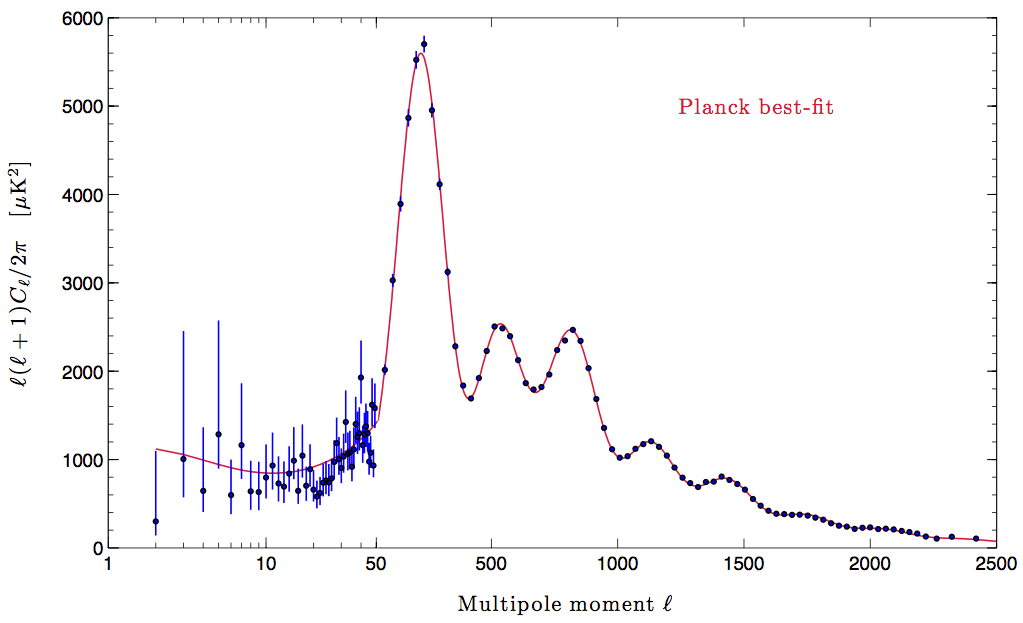
\includegraphics[width=\linewidth]{cmb/images/mission_spectrum.png}
	\caption{Leistungsspektrumsanalyse von der ESA durchgeführt. 
	\ref{bib:cmb_spectrum_esa}}
	\label{fig:cmb-power-spec-1200}
\end{figure}